Este capítulo tem como propósito fornecer o embasamento teórico necessário 
para o entendimento da construção do sistema proposta. Aqui é contido uma
descrição detalhada das técnicas, métodos e tecnologias utilizadas, assim  
preparando o leitor para o conteúdo dos próximos capítulos.


\section{Design de APIs}
Separação de conceitos, traduzido do termo \emph{Separation of Concerns}, é uma temática 
chave na arquitetura cliente-servidor da internet. Parte do porquê a internet funciona tão bem
foi a preocupação, desde sua concepção, de uma interface uniforme que, desde que respeitada, 
 daria liberdade aos desenvolvedores de implementar, em qualquer linguagem ou tecnologia,
 um de seus componentes. 

Apesar do sucesso na separação de conceitos entre as responsabilidades que o navegador 
e o servidor empregam, a mesma preocupação não foi replicada entre interfaces e 
funcionalidades que o servidor expõe. 
Com frequência existe um alto acoplamento entre a interface, \emph{Frontend},
e o servidor, \emph{Backend}, o que resulta em uma interface não uniforme para interação 
dos recursos que deveriam estar expostos. Define-se aqui um recurso como qualquer conceito 
na internet que pode ser referenciado por um identificador único e manipulado por uma interface uniforme 
\ \cite{masse2011rest}.

A solução, que leva ao desacoplamento, é a interação com estas
funcionalidades través de uma \emph{API}, \emph{Application Programming Interface},
exposta pelo \emph{backend}, que provê formas padronizadas 
de acesso. Aqui não somente ganhamos portabilidade, já que possibilitamos que não só 
um tipo de cliente, navegadores, saibam como acessar nossos recursos, mas ganhamos espaço 
para criar uma camada de abstração do serviço \emph{Web}, modelando-o em recursos.
Estes recursos não serão projetados como uma cópia da organização de dados ou funcionalidades 
presentes no \emph{backend} mas em representações que sejam de fácil consumo e de entendimento 
ubíquo pelo lado do cliente.

O desafio de criar bons serviços na internet pode ser facilitado se empregarmos estilos 
arquiteturais já existentes. Aqui definimos estilos arquiteturais como 
um conjunto coordenado de restrições arquiteturais. \\
Um destes estilos arquiteturas que tem ganhado cada vez 
mais tração se chama \emph{REST}, \emph{Representational State Transfer}, ou em português,
\emph{Transferência Representacional de Estado}. Cunhado por \citeonline{fielding2000architectural}, 
o termo evoca como uma sistema na \emph{Web} deveria se comportar, uma máquina de estados 
virtuais em que o usuário progride através da seleção de identificadores únicos, que identificam 
recursos, e verbos \emph{HTTP}
que operam sobre estes recursos.

As restrições na arquitetura impostas pelo estilo \emph{REST} são agrupadas em seis categorias:
\begin{description}
\item[Cliente-servidor:] A separação dos papéis do cliente e servidor deve ser clara para 
  que estes possam ser projetados e implementados de forma independente. A interação 
  entre eles só acontece na forma de requisições, que são iniciadas pelo cliente. 
  Servidores devem mandar respostas apenas como reações de requisições dos clientes.
\item[Interface uniforme:] interfaces \emph{REST} possuem quatro  restrições:
identificação de recursos, manipulação de recursos através de representações, 
mensagens auto-descritivas e hipermídia como motor de estado da aplicação, \emph{HATEOAS}.\\
A primeira dita que cada recurso precisa ser enderessável 
por um identificador único, \emph{URI}, \emph{Unique Resource Identifier}.\\
Este 
recurso pode ser representado de diversas formas, seja um \emph{HTML}, que é mais adequado para 
um navegador,
ou \emph{JSON} que é mais apropriado para consumo de outro programa. Percebe-se aqui 
que a representação é apenas uma forma de interagir com o 
recurso,  não o próprio recurso. Isto é o que dita a segunda regra. \\
No consumo de um \emph{API}, o cliente especifica um recurso e seu estado 
desejado, enquanto o servidor deve responder com o recurso e seu estado real. 
Esta troca de mensagens  deve ser feita utilizando \emph{headers} e 
códigos de estado \emph{HTTP} que descrevam o estado 
do recurso e metadados correspondentes, de forma que as mensagens sejam auto-descritivas.\\
A última restrição, \emph{HATEOAS}, ajuda a aumentar a visibilidade e descoberta de recursos 
relacionados na \emph{API}, que ajudam o cliente a navegar dinamicamente nos recursos expostos.
Assim, quando referenciam-se outros recursos, também são fornecidos seus identificadores únicos 
e verbos aceitos para aquela rota.
\item[Sistema em camadas:] Restringe-se o comportamento dos componentes em camadas, em que 
  cada camada só pode interagir com subjacentes. 
  Entre as chamadas do cliente que requisita uma representação de um estado de um recurso, e 
  o servidor que processa a requisição, podem haver vários servidores entre eles. Estes 
  servidores podem prover um camada de segurança, \emph{cache}, balanceamento de carga ou 
  outras funcionalidades. Estas camadas não devem afetar a requisição ou resposta e nem o cliente 
  nem servidor precisam estar cientes se elas existem ou não.
\item[Protocolo sem estado:] O servidor não deve lembrar absolutamente nada do usuário que 
  utiliza sua \emph{API}. Isto implica que toda requisição individual precisa conter toda 
  informação necessária para que o servidor processe e retorne uma resposta. Esta restrição 
  visa aumentar a escalablidade, visibilidade e confiabilidade do sistema. Escalabilidade pois 
  permite que haja \emph{caching} de respostas e que o servidor possa desalocar recursos 
  físicos entre requisições, visibilidade pois sistemas que monitoram requisições não 
  precisam olhar além de uma requisição, pois elas contém todo o dado necessário 
  para entender a natureza desta, e a confibilidade pois a recuperação de falhas 
  parciais se torna mais simples \ \cite{kendall1994note}.
\item[Cache:] O servidor deve declarar quais dados podem ser guardados em \emph{caches}. 
  \emph{Caches} ajudam a reduzir a latência percebida pelo cliente, aumentam a disponibilidade 
  e confiabilidade de serviços e mitigam a carga de trabalho do servidor. Em resumo, 
  \emph{caches} reduzem todos os custos associados a um serviço na \emph{internet}.
\item[Código sob demanda:] A internet faz bastante uso de código sob demanda, que possibilita 
  que o servidor transfira executáveis, tais como \emph{scripts} e \emph{plugins}, para a 
  execução do lado do cliente. Apesar de proposto por \citeonline{fielding2000architectural}, 
  esta restrição tende a estabelecer um acoplamento de tecnologias entre servidor e cliente. 
  Por este motivo ``código sob demanda'' é a única restrição imposta pelo estilo arquitetural 
  \emph{REST} que é considerada opcional.
\end{description}

O maior desafio no projeto de uma \emph{API} é abstrair componentes do sistema
em recursos. O modelamento destes recursos estabelece os aspectos chaves da sua \emph{API}
e é semelhante ao processo de modelar um banco de dados relacional ou mesmo o modelamento 
clássico de um sistema orientado a objetos.

No processo de modelagem de recursos, rotineiramente começa-se pensando em arquétipos de 
recursos. Estes arquétipos nos ajudam a  comunicar de forma consistente 
as estruturas que são frequentemente encontradas em \emph{Designs} de \emph{REST APIs}.
Idealmente, cada recurso pertencerá a apenas um dos seguintes arquétipos: \emph{document}, 
\emph{collection}, \emph{controller} e \emph{store}.

\emph{Document} é o arquétipo base de todos os outros, todos os outros arquétipos são especializações 
destes. Sua representação tipicamente incluí campos com dados ou \emph{hiperlinks} para outros 
recursos. \emph{Collection} é um diretório de outros recursos em que clientes podem recuperar 
ou, possivelmente, adicionar novos items a coleção. Já \emph{Stores} são recursos que permitem 
que usuários guardem novos recursos, de forma que o próprio cliente escolha o 
identificador daquele recurso. Para recursos que se parecem mais como procedimentos que 
não se encaixam nos métodos padrões, \emph{CRUD} (\emph{create, retrieve, update, delete}),
  o arquétipo \emph{Controller} é adequado. Todos estes arquétipos 
  contém recomendações de como o identificador único deve ser escolhido, para que seja 
  claro a quem consome a API de qual arquétipo se trata aquele recurso.

  \section{O padrão \emph{OAuth}}
  Apesar de vivermos em um mundo que depende, cada vez mais, de serviços digitais,
  a maior parcela dos usuários ainda não se educaram ou 
  não seguem boas práticas de segurança na \emph{internet}. Não é infrequente que se 
  use as mesmas credenciais em múltiplos serviços, mesmo que o usuário 
  não tenha meios de averiguar que suas informações são manuseadas e armazenadas de forma 
  adequada.

  Uma das possíveis soluções para uma melhor gestão de identididade na \emph{internet}, 
  é o uso de identidades federadas \cite{208723}. Uma identidade federada é um meio 
  de uma pessoa vincular sua identidade eletrônica e atributos pessoais 
  a múltiplas partes distintas. Esta solução trás benefícios como mais garantias
  de segurança no armazenamento de credencias, menos sobrecarga de responsabilidade 
  para desenvolvedores de aplicações e uma melhor experiência para o usúario, já que se 
  diminuí o atrito na criação e gerenciamento de múltiplas contas.

  O modelo de serviço federado pode ser dividido em duas componentes necessárias: 
  o provedor de identidade e o provedor de serviço. Ambas as partes cumprem papéis 
  distintos e sem qualquer uma delas não temos uma solução de identidade federada. 
  Para que a solução funcione, deve se haver um relacionamento de confiança entre 
  o provedor de identidade e o provedor de serviço. Caso o provedor de identidade 
  não confie no provedor de serviço, este não o confiará os dados de usuários.
  Caso o provedor de serviço não confie no provedor de identidade, 
  também não confiará nas informações advindas dele.

  O provedor de identidade é quem mantém as informações de identidade. Usuários 
  se autenticam diante ao banco de credenciais do provedor, que então libera as
  informações relativas àquele usuário ao provedor de serviço que iniciou o processo 
  de autenticação. O provedor de serviço é aquele que provê serviços a usuários, 
  estes sendo aplicações, serviços de infraestrutura ou serviços de dados. Com a popularização 
  do modelo de computação em nuvem, cada vez mais usuários entram em contato com algum dos três 
  principais modelos de serviço em nuvem,  \emph{Infrastructure as a Service} (\emph{IaaS}), 
  \emph{Platform as a Service} \emph{PaaS} e \emph{SaaS}, \emph{Software as a Service}, 
  todas as quais depende de um modelo de serviço federado \cite{rountree2012federated}.

  Existem vários padrões que implementam o modelo de serviço federado, as mais famosas sendo:
  \emph{SAML} (Security Assertion Markup Language), \emph{OAuth}, \emph{OpenID}, 
  \emph{Simple Web Tokens}, \emph{JSON Web Tokens} e \emph{Windows Identity Foundation}. O 
  padrão que tem ganhado mais adeptos, pela sua abordagem simples porém robusta,
  é o padrão \emph{OAuth}, que já conta com quatro revisões, sendo a última
  \emph{OAuth 2.0}. 

  \emph{OAuth 2.0} é um padrão aberto criado para suportar autorização de forma segura. 
  Existem três papéis definidos pelo padrão: servidor de autorização, servidor de recurso e 
  dono do recurso. Em modelos tradicionais cliente-servidor, o dono do recurso, ou seja, cliente 
  acessaria recursos no servidor de recurso, desde que este consiga se autenticar com 
  sucesso no servidor. No padrão \emph{OAuth} temos duas ou três partes envolvidas, 
  sendo duas quando o servidor de autorização também é o dono do recurso.

  \emph{OAuth 2.0} suporta vários fluxos de autenticação: fluxo usuário-agente, 
  fluxo servidor \emph{Web}, fluxo de dispositivo, fluxo de usuário e senha, fluxo 
  de credencias de cliente e fluxo de asserção. A maioria das aplicações \emph{Web}, 
  principalmente quando se tratam de \emph{Single Page Applications},
  fazem uso do fluxo servidor \emph{Web}, também 
  conhecido por ``concessão de código de acesso" (\emph{Authorization Code Grant})
  que é ilustrado pela \fref{fig:web_flow} e definido por \citeonline{hardt2012rfc}. 

  O fluxo de concessão de código de acesso começa quando um usuário, dono de um recurso, escolhe 
  fazer \emph{login} ou atrelar sua conta do servidor de autorização em uma aplicação. A aplicação 
  faz uma requisição ao servidor de autorização que por sua vez retorna uma página de \emph{login}. 
  O usuário preenche suas credencias na página e autoriza a aplicação a acessar um determinado 
  escopo de recursos. Em seguida, o servidor de autorização emite um código de autorização, 
  que geralmente expira em minutos. A aplicação, em posse do código de autorização, requisita 
  ao servidor de autorização um código de acesso. Com o código de acesso, a aplicação agora 
  pode acessar recursos protegidos do servidor de recursos, até que este código expire.

  Existem alguns detalhes que garantem a segurança do fluxo anterior. Quando a aplicação requisita 
  o servidor de autorização por um código de autorização, ela informa um identificador de cliente, que 
  indica sua identididade, uma \emph{url} de retorno, que é para aonde o servidor de autorização mandará 
  o código de acesso e uma cadeia de caracteres aleátorios que será usado para validar se a requisição 
  veio do servidor de autorização. Caso na requisição a \emph{url} de retorno informada seja diferente 
  da cadastrada pela aplicação no servidor de autorização previamente, a requisição é abortada. No 
  recebimento da resposta do servidor de autenticação, caso a cadeia de caracteres aleátorios não seja a mesma 
  da enviada, aborta-se o processo. Para obtenção do código de acesso, a aplicação também não somente deve informar 
  ao servidor de autenticação o código de autorização, mas também um segredo previamente cadastrado em conjunto 
  com seu identificador.
  \begin{figure}[htpb]
    \centering
    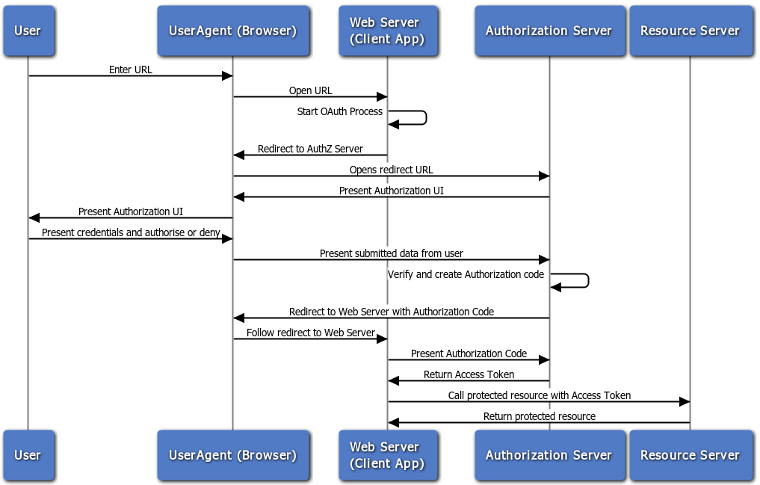
\includegraphics[width=0.95\linewidth]{images/web_flow.png}
    \caption{Diagrama que explica o funcionamento do fluxo servidor \emph{Web}, 
      definido na seção 4.1 da norma \emph{RFC 6749}, retirado de \url{https://www.authlete.com}.}%
    \label{fig:web_flow}
  \end{figure}
  

  \section{Integração e entrega contínua}
  Um dos grandes desafios no desenvolvimento de \emph{software} é criar um processo repetível e 
  confiável para entregas de aplicações. Frequentemente, lançamentos de \emph{software} são
  tratados por seus desenvolvedores como momentos estressantes. Associa-se este \emph{stress} a
  muitos processos manuais, infrequentes e propensos a erros, conduzidos em curtos prazos 
  de tempo.
  
  Pode-se, no entanto, se um processo rigoroso for seguido,  
  tornar esta tarefa fácil, tão fácil quanto o apertar de um botão.
  Para atingirmos este nível de maturidade no desenvolvimento de 
  \emph{software}, \citeonline{humble2010continuous} propõe que
  devemos seguir a risca dois princípios: automatização de todas etapas que sejam 
  automatizáveis e manter todos os artefatos necessários para um lançamento em um sistema de 
  controle de versões. 

  Idealmente, uma entrega de \emph{software} é composta por três coisas: 
  provisionar e gerenciar um ambiente que a aplicação irá rodar (configuração de \emph{hardware},
  \emph{software}, infraestrutura e serviços externos), instalar a versão correta da aplicação 
  neste ambiente e configurar a aplicação, incluindo qualquer estado ou dado que ela possa requerer.

  De fato, até recentemente, vários destes passos para a entrega de \emph{software} pareciam 
  impossíveis ou ao menos complexas de aderirem os princípios citados por 
  \citeonline{humble2010continuous}. Como poderíamos, por exemplo, 
  versionar \emph{hardware}? Com o advento de virtualização eficiente e barata, até esta 
  tarefa que, \emph{a priori}, parecia impossível, virou algo corriqueiro e ubíquo. 
  Com advento e adoção da computação em nuvem, todos os passos necessários para automatização 
  de testes, compilação ou de artefatos e lançamento do \emph{software} estão 
  acessíveis a qualquer desenvolvedor.

  Define-se integração contínua como o processo no desenvolvimento de \emph{software} em que 
  membros de um time integram seu trabalho de forma frequente. Cada integração desencadeia etapas 
  como verificação de estilo de código, testes automatizados e construções de compilados ou 
  outros artefatos, com o objetivo de encontrar problemas nas integrações o mais rápido possível.
  Já entrega contínua leva a prática de integração contínua para outro patamar e automatiza 
  o lançamento de versões do \emph{software} dado que as etapas anteriores foram concluídas com 
  sucesso e o código foi revisado \cite{fowler2006continuous}.
